\chapter{Diseño}\label{cap:disenio}

En este capitulo se documentara como se desarrollo el diseño de la arquitectura del proyecto, para ello se expondrá el modo en que trabaja \jd y además se mostrara la estructura de clases que se eligió para el sistema para que pueda cumplir con los requisitos expuestos en el Capitulo \ref{capitulo:especificacion}.





\section{Visión general}

Para diseñar \jj como ya se menciono se tomo como base a el patrón de desarrollo DAO que se explico en la sección \fullref{jdbgm:dao}, siguiendo la idea de este patrón \jj debe manejar todas las consultas echas a el motor por lo que la aplicación solo se deberá comunicar con \jj para acceder a el motor de base de datos, se puede observar esquemáticamente esta idea en la figura \figpage{fig:jdbgm:overview} en la que podemos observar que la idea es que la aplicación utilice el formato que estamos proponiendo para trabajar con las sentencias SQL, estas serán interpretadas por \jj y convertidas a una cadena de texto la cual es entendible por \jd y este se comunicara directamente con el DBMS y pondrá a disposición de \jj el resultado que dependiendo de la consulta puede ser un objeto del tipo \verb=ResultSet= o un tipo \verb=integer=. 

\begin{figure}
  \centering
    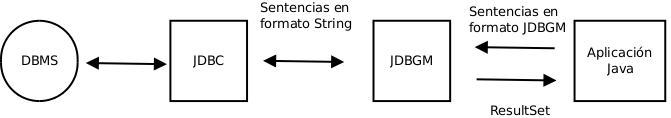
\includegraphics[width=0.85\textwidth]{figuras/jdbgm-overview.png}
  \caption{JDBGM dentro de una aplicación}
  \label{fig:jdbgm:overview}
\end{figure}

Así que \jj debe ser capaz de hacer dos tareas independientes pero relacionadas, en primer lugar debe proveer el almacenamiento de las sentencias de modo que puedan ser traducidas luego a el dialecto que corresponda y en segundo lugar proveer los métodos necesarios para comunicarse con el motor mediante \jd, podemos observar esquemáticamente la situación en la figura \figpage{fig:jdbgm:closerlook} que nos muestra la idea de independencia existente entre los dos módulos principales que se están exponiendo, el manejador de sentencias es totalmente independiente de la capa intermedia pues de lo que esta encargado es de proveer los métodos necesarios para ``armar las sentencias'' y traducirlas cuando sea requerido a el dialecto correspondiente, esta traducción lo que hace es convertir la sentencia almacenada a una cadena de texto la cual es entendible por \jd por lo que se podría obviar la capa intermedia que hace transparente su uso y usarlo directamente. En cambio la capa intermedia dependerá de el manejador de sentencias para poder proveer la independencia de dialectos que se quiere lograr y además este solo recibirá las sentencias compatibles con el formato propuesto por \jj por lo que a continuación se procederá a explicar la estructura propuesta para este manejador para que después se pueda explicar correctamente el funcionamiento de la capa intermedia.

\begin{figure}
  \centering
    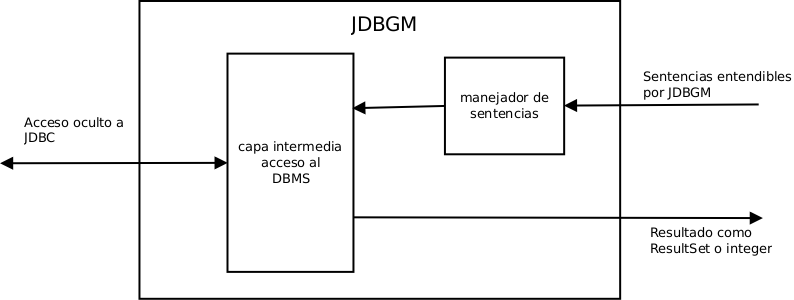
\includegraphics[width=0.85\textwidth]{figuras/jdbgm-closerlook.png}
  \caption{Vista abstracta del funcionamiento de JDBGM}
  \label{fig:jdbgm:closerlook}
\end{figure}

\section{Manejador de sentencias}
Como ya se dijo el manejador de sentencias debe ser capaz de almacenar las sentencias de forma desglosada así que pasemos a ver que se quiere lograr. Como una primer solución podemos pensar que una sentencia como la siguiente ``\verb=nombre_comando parametro opcion1 parametro1 opcion2 parametro2='' que se podría corresponder con la siguiente consulta ``\verb|SELECT * FROM table WHERE table.id=1|'', salvando ciertas reglas de construcción que en este momento no vienen al caso, puede ser almacenado en una clase que se corresponda con el siguiente esquema:

\begin{lstlisting}[title=Pseudocódigo de la estructura de dato que contiene la sentencia]
class Sentencia{
	nombre_comando;
	parametro;
	set_opcion1(parametro1);
	set_opcion2(parametro2);
	devolver_sentencia();
}
\end{lstlisting}
Como se ve es una idea bastante sencilla en la que la clase identificara la sentencia y sus opciones correspondientes serán nombres de atributos pues en definitiva lo que nos interesa de estas opciones son los valores que toman o si están presentes o no en la sentencia que se esta armando. Como clase de POO también debe ofrecer métodos para almacenar los valores que tomaran las opciones y es aquí donde empiezan a jugar las reglas dispuestas en el dialecto genérico que fue especificado en el capitulo \ref{capitulo:especificacion}, puesto que las opciones ofrecidas por cada sentencia no pueden ser libremente usadas es necesario que estos métodos restrinjan el modo en que se pueden usar ya sea limitando las posibilidades de el/los métodos o bien usando excepciones para detener la ejecución del programa, una explicación mas detallada del manejo de excepciones se vera en las secciones siguientes, cuando alguna acción ilegal sobre las sentencias ocurra.

Con esto ya se tiene una idea genérica de las clases que se quiere representen a las sentencias y teniendo en cuenta que cada una de estas clases representa a una sentencia diferente con un comportamiento diferente pero con similitudes es necesario recalcar que estas diferentes clases deben presentar las mismas similitudes, por ejemplo supóngase que los objetos \verb|select| y \verb|create| representan las sentencias SQL del mismo nombre las cuales precisan que se les asigne el nombre de la tabla sobre la que se esta trabajando entonces lo correcto sera que ambos objetos tengan un método de igual nombre y comportamiento igual como por ejemplo \verb=select.set_table_name("name_1")= y \verb=create.set_table_name("name_2")=. Es muy importante tener en cuenta esto puesto que facilitara el aprendizaje del uso de la API del manejador de sentencias que se esta proponiendo y además hará el uso de la misma mucho mas natural, con respecto a SQL. Antes de empezar a hablar de lleno de la arquitectura propuesta para el manejador de sentencia es necesario nombrar al paquete \cc de el cual se tomaron algunas ideas.

\subsection{El paquete \cc}
Este paquete que puede ser encontrado en \href{http://sourceforge.net}{SourceForge} en la siguiente dirección \url{http://sourceforge.net/projects/crossdb/} intenta solucionar el mismo problema que el manejador de sentencias aquí presentado tal como se puede observar en la pagina del proyecto que se resume en la siguiente oración:

\begin{center}
``To provide cross database tools for manipulating all major databases without having to worry about each vendors specific implementation.''
\end{center} 

Esta librería  usa la misma idea de ir generando bajo demanda las sentencias por lo que se la estudio y se llego a la conclusión de que podía servir como base para el manejador que se quiere implementar en este proyecto. Algunas consideraciones antes de avanzar:
\begin{itemize}
\item El paquete se distribuye bajo Apache Software License 1.1 por lo que no hay inconvenientes en reusar el código escrito, siempre y cuando se respeten las condiciones impuestas. Además esta licencia es compatible con GPL.
\item La ultima actualización del proyecto data el 23-08-2005 (la ultima modificación registrada en el repositorio svn) por lo que aparentemente el proyecto quedo en un punto muerto y en una versión beta básica según se puede ver al revisar el código.
\item Carece de una buena documentación pero el código es bastante entendible y mas aun después de venir estudiando una solución similar a la propuesta por \cc


\end{itemize}
Se puede resumir la estructura usada por esta librería en el gráfico \fullref{fig:crossdb:base-idea} que nos muestra que por cada sentencia existe una Interfaz \verb=Statement= que define el comportamiento de la misma, luego para esta interfaz base existe una implementación por defecto \verb=DefaultStatement= que implementa las funciones que son comunes a toda implementación que se pueda realizar de dicha interfaz, recordando que al trabajar con dialectos estamos trabajando con variaciones de un lenguaje base, y por cada una de estas implementaciones por defecto existe una implementación especifica \verb=SpecificStatement= que contempla las particularidades de un motor en particular sobre dicha sentencia. En la misma figura podemos observar como se conforma dicha arquitectura para la sentencia \verb=SELECT= con la clases \verb=SelectQuery= siendo la interfaz base, \verb=DefaultSelectQuery= siendo la implementación por defecto de dicha interfaz y \verb=OracleSelectQuery= una implementación especifica para el dialecto usado por Oracle.


%\begin{figure}
%  \centering
%    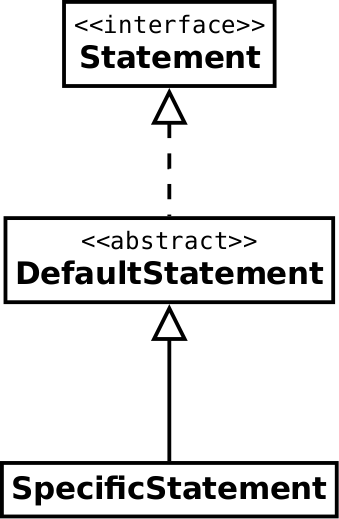
\includegraphics[width=0.2\textwidth]{figuras/crossdb-base-idea.png}
%  \caption{Vista abstracta de la arquitectura de crossdb}
%  \label{fig:crossdb:base-idea}
%\end{figure}
\begin{figure}
  \centering
  \subfloat[Idea base]{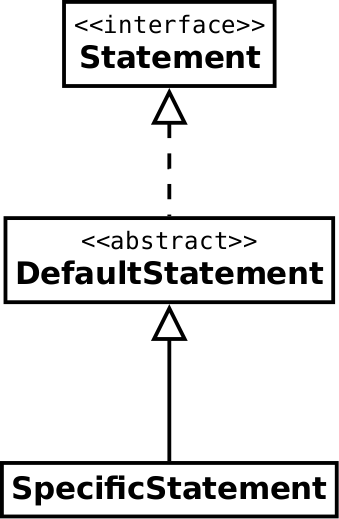
\includegraphics[width=0.2\textwidth]{figuras/crossdb-base-idea.png}} \label{fig:subfig:crossdb:base-idea}
  \qquad 
  \subfloat[Ejemplo con Select]{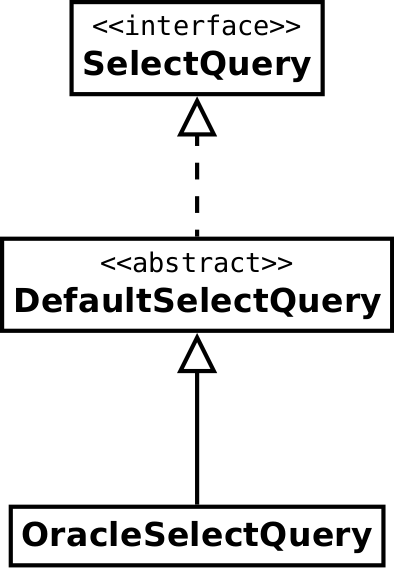
\includegraphics[width=0.2\textwidth]{figuras/crossdb-base-idea-select.png}} \label{fig:subfig:crossdb:base-idea-select}
  \caption{Vista abstracta de la arquitectura de crossdb}
  \label{fig:crossdb:base-idea}
\end{figure}

Además de las clases a las que se hizo referencia \cc usa otras auxiliares, como \verb=Column= que contiene los datos necesarios para especificar una columna o \verb=WhereClause= que representa una clausula \verb=WHERE=, necesarias para poder almacenar adecuadamente los datos para las sentencias que se están armando. También se implementa la idea del patrón Factory pero de una manera muy básica. Terminado de presentar ligeramente este paquete sobre el cual se baso el diseño propuesto en este trabajo se pasara a exponer la arquitectura usada por el manejador de sentencias y su relación con las ideas tomadas de \cc.

\subsection{Diseño básico de el Manejador}
%Para la implementación de las especificaciones declaradas anteriormente nos encontramos con que existen algunas similitudes entre las diferentes clases definidas anteriormente, atendiendo a que cada clase representa a una de las sentencias SQL que se incluyeron en el proyecto y cada clase esta compuesta por:
Recordando lo expuesto en la sección anterior sobre las clases que representan las sentencias podemos resumir su contenido de manera muy genérica de la siguiente manera:

\begin{itemize}
\item Variables que almacenaran los datos necesarios para la construcción de los métodos, aunque también puede ser necesario el uso de clases auxiliares dependiendo de la complejidad de la clase.

\item Métodos para inicializar la clase y agregar (lo que comúnmente se dice \textit{setear}), es decir poblarla con los datos necesarios para su construcción.

\item Un método para armar la sentencia.

\end{itemize}

La estructura de cada una de estas clases puede ser implementada directamente desde las restricciones impuestas en la sección \fullref{seccion:especificacion:dialectos} pero siguiendo ciertos lineamientos que veremos a continuación.

En primer lugar se tiene que tener en cuenta la arquitectura general de el manejador para ello hay que observar lo siguiente: se puede hacer una distinción en como es que responde el motor de base de datos a las sentencias, o mas bien como responde JDBC, que es el "interlocutor" cuando procesa determinada sentencia SQL. Por un lado están aquellos que solo necesitan reportar la cantidad de filas afectadas por la sentencia después están aquellos que necesitan devolver información después de ejecutada la sentencia, estas ultimas sentencias son precisamente las que realizan consultas sobre la base de datos siendo las sentencias \verb=SELECT= las únicas que hacen esto. Por otro lado las sentencias \verb=UPDATE=, \verb=INSERT= y \verb=DELETE= solo precisan reportar la cantidad de filas que fueron afectadas por la consulta, en cambio las sentencias \verb=ALTER TABLE= y \verb=CREATE TABLE= que sirven para modificar las tablas (son parte del DDL de SQL) no afectan directamente a las filas de la misma pero por convención se tomo que \jd devuelva 0 como numero de columnas afectadas por lo que en este caso se las agrupara en el mismo conjunto. Entonces para que \jj pueda hacer distinción de estos dos tipos de consultas se utilizaron dos interfaces las cuales pueden ser tomadas como tipos genéricos, la \figpage{fig:crossdb-base} muestra estas interfaces y sus hijas.

\begin{figure}
  \centering
    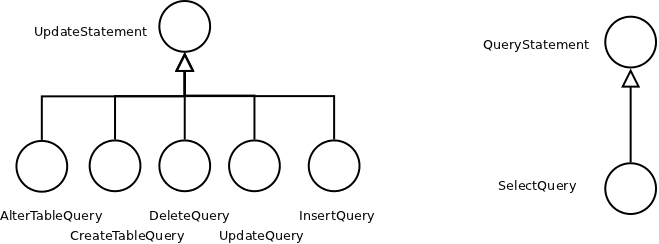
\includegraphics[width=0.65\textwidth]{figuras/crossdb-base.png}
  \caption{Interfaces base para los tipos de sentencia}
  \label{fig:crossdb-base}
\end{figure}

De este modo se utilizan las interfaces \verb=UpdateStatement= y \verb=QueryStatement= como un tipo genérico para identificar las sentencias que no realizan consultas de aquellas que si, es decir si en la firma de cualquier método se declara algo similar a lo siguiente \verb=metodo_a(UpdateStatement statement)= el parámetro \verb=statement= podrá ser cualquier clase que sea heredera directa o indirectamente de la interfase \verb=UpdateStatement= y no podrá tomar ninguna heredera de la clase \verb=QueryStatement=, en este caso la herencia de la interfaz base sera indirecta como se aclarara a continuación y además cabe aclarar que este es el primer cambio que se agrego a la estructura que proponía \cc.

\begin{figure}
  \centering
    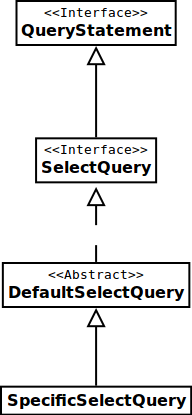
\includegraphics[width=0.65\textwidth]{figuras/crossdb-query.png}
  \caption{Diagrama de clases para la sentencia SELECT}
  \label{fig:query-base}
\end{figure}

En la \figpage{fig:query-base} tenemos una vista completa de como se debe componer la estructura de clases para el tipo base \verb=QueryStatement=, que es la mas simple pues solo tiene una clase hija, la única que sirve para hacer consultas sobre la base de datos la sentencia \verb=SELECT=. Como ya se dijo la primer interfase sirve para distinguir a nivel genérico el tipo de sentencia SQL que se esta tratando, la interfase hija directa de \verb=QueryStatement= si ya define un comportamiento especifico para las funciones de las sentencias \verb=SELECT=. La clase abstracta \verb=DefaultSelectQuery= brinda una implementación base para los métodos definidos en \verb=SelectQuery=, para comprender por que se debe hacer esto es necesario recordar que la clase que represente una sentencia contiene toda la información necesaria para generar una sentencia valida y esta información es la misma que se precisa para cualquier sentencia SQL de un dialecto en concreto (además ya se definió una sintaxis que es totalmente soportada) la diferencia esta en el modo que se escriben las sentencias, la sintaxis, por ello el único método que deberá ser especifico a un \dd será aquel que esta encargado de armar la sentencia. Después de la clase abstracta si por fin tenemos implementaciones especificas para cada uno de los motores, estas son la clase \verb=SpecificSelectQuery=de las que se hablaba en la \figpage{fig:crossdb:base-idea}, la idea es que de estas clases hayan tantas como motores estén soportados por el proyecto.

\begin{figure}
  \centering
    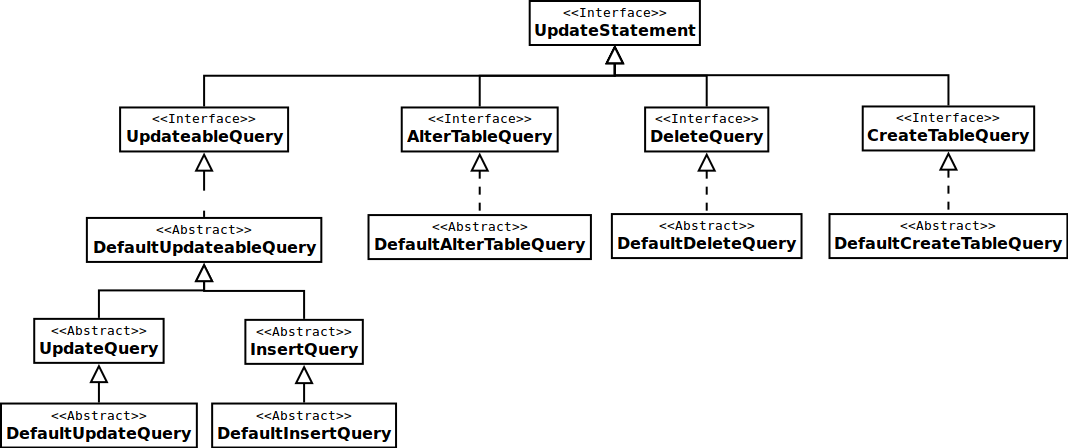
\includegraphics[width=\textwidth]{figuras/crossdb-update.png}
  \caption{Estructura de las otras sentencias}
  \label{fig:update}
\end{figure}

En la \figpage{fig:update} tenemos una descripción de como se deben estructurar los tipos de la interfaz base \verb=UpdateStatement=, esta es algo mas elaborada pero como antes la primer interfaz, funciona como tipo genérico, en las clases hijas de esta vemos algo parecido al caso de \verb=QueryStatement= salvo por la interfaz \verb=UpdateableQuery= que agrupa comportamiento común a \verb=Updatequery= e \verb=InsertQuery=, también se brinda un comportamiento predeterminado para esta mediante \verb=DefaultUpdateStatement= pero el cual al brindar una implementación base tiene que ser a la fuerza una clase abstracta\footnote{Una clase abstracta se puede ver como una interfaz que fuerza la implementación de parte de su comportamiento} así que las clases que definen el comportamiento especifico de \verb=UpdateQuery= e \verb=InsertQuery= son clases abstractas y no interfaces, pero el resultado es el mismo. Y finalmente para cada una de las interfaces que definen(o representan) a las sentencias tenemos una implementación por defecto en las clases cuyo nombre empieza por \verb=Default= de las cuales deberán heredar cada una de las implementaciones especificas, en la figura \ref{fig:update} no se las representa puesto que seria demasiado extenso.

Después de analizar el dialecto genérico que se definió en la sección \fullref{seccion:especificacion:dialectos} y de definir la estructura de las clases para el manejador se buscaron aquellos atributos de las clases (extraídos de las sentencias que representan) que por su complejidad ameritaban convertirse en una clase por si mismas, tal es el caso de una columna que en si es una entidad distinguible y lo suficientemente compleja como ejemplo podemos notar que una columna posee nombre, tipo de dato que almacena y muchas otras restricciones que pueden ser encontradas en el capitulo \ref{cap:disenio} en la sección que se refiere a la sentencia \verb=CREATE TABLE=. A continuación se listan y explican las clases auxiliares que se encontraron. 

%un análisis mas detallado de como se componen las interfaces finales y las clases que las implementan además de una vista a su implementación y las clases que sirven como componente de las principales.
\subsection{Clases Auxiliares} \label{seccion:disenio:clases-auxiliares}
Como ya se denoto para un adecuado y consistente funcionamiento de el manejador de sentencias es necesario crear algunas clases extras que brindan funcionalidades comunes a varias clases o bien funcionalidades extras no propias de dichas clases que ayudaran a formar las similitudes entre las diferentes clases que representan a las sentencias, a continuación un listado de estas:

\begin{itemize}
\item \verb=Column=
\item \verb=TableConstraint=
\item \verb=DataTypes=
\item \verb=Formater=
\item \verb=Functions= (no decidido por completo)
\item \verb=Join=
\item \verb=SpecificSQLFactory=
\item \verb=SQLFactory=
\item \verb=SQLFormat, SQLDateTimeFormat, SQLTimeFormat=(estas no son usadas o movidas a Formatter)
\item \verb=WhereClause, WhereCondition, WhereFrame=
\end{itemize}
A continuación una descripción de ellas

\subsubsection{La clase Column}
Representa una columna de una tabla para ello posee atributos tales como nombre de columna, banderas que indican si es clave foranea y todos los demás atributos que sirven para definir la columna en una sentencia \verb=CREATE TABLE=. Entre sus métodos no se incluye ninguno que sirva para convertir la columna en una cadena  de texto que sirva para definirla en una sentencia SQL pues a pesar de que la sintaxis de la definición de columna no varia demasiado, salvo por los tipos de datos, si varia el uso sobre ella pues la sentencia \verb=ALTER TABLE= también puede definir columnas en su sintaxis pero con ciertas restricciones como se ve en la sección \ref{sec:altertable} y para evitar confusiones cada clase (clase que represente una sentencia) que haga uso de un objeto columna deberá implementar las restricciones sobre la construcción de la sentencia ignorando los atributos que no use.

Además de esto la columna también posee un atributo para almacenar un valor para la columna de modo que la clase no solo sirva para definir una columna si no también como contenedor del valor, del tipo y del nombre  de la columna para usarlo luego con otras sentencias que no necesiten definir columnas si no ingresarles datos como es el caso de \verb=INSERT=. Haciendo esto se evita crear otra clase que solo sirva de contenedor para el valor de una columna y por lo tanto hay menos clases para recordar. Además se deja abierta la posibilidad de establecer a que tipo de datos pertenece el valor que se esta ingresando para poder manejar el modo en que este valor es convertido a \verb=String=, para aclarar esto supóngase que se quiere ingresar un valor booleano a una columna y como los constructores de esta clase aceptan para el parámetro que establece el valor para la columna un objeto de la clase \verb=Object= se le puede pasar cualquier objeto por lo que intuitivamente se le podría pasar una cadena \verb|columnValue ="TRUE"| a menos que se indique el tipo de columna a la clase la clase puede inferir que se quiere enviar una cadena de texto y convertirla a  por ejemplo \verb|.. SET boolean_column = 'TRUE'| que puede llevar a un error cuando se intente enviar la sentencia a el motor, en cambio si el tipo de dato es establecido a boolean la clase lo convertirá en un \verb=1= o \verb=0= según corresponda.

\subsubsection{Las restricciones de tabla en TableConstraint}
Esta clase representa lo que en una sentencia \verb=CREATE TABLE= vendría a ser una restricción de tabla, las cuales pueden ser \verb=PRIMARY KEY, FOREIGN KEY o UNIQUE= estas restricciones a su vez pueden hacerse sobre una (clave simple) columna o bien sobre varias (clave compuesta). La razón por la que se eligió crear una clase para representar las restricciones de tabla es que de no existir se complicaba mucho la "traducción" a SQL de la clase que representa a \verb=CREATE TABLE=, esta clase representa un medio mas sencillo para la traducción de la restricción, como contra parte se puede observar que la sintaxis se vuelve un poco mas compleja pero aun así es mayor el beneficio pues se hace mas sencilla la traducción a cadena de caracteres. 

\subsubsection{La clase DataTypes}
Esta es una clase abstracta que servirá para mapear los tipos de datos a los correspondientes a los de un motor especifico, esto se logra mediante un método que toma como entrada los tipos de datos definidos por \jd y los mapea a los tipos de datos encontrados en el capitulo anterior.


\subsubsection{La interfaz Formatter}
La Interfaz \verb=Formatter= sirve para definir el modo en que algunos tipos de datos han de ser convertidos a su equivalente como cadena de caracteres, se puede decir que define un formateador. Se provee una implementación por defecto de esta interfaz en \verb=DefaultFormatter= la cual puede llegar a servir sin modificaciones para el motor sobre el que se este trabajando, aun así esta implementación por defecto obligara a que se cree una clase que herede de la misma puesto que se tratara de una clase abstracta y como tal no puede ser instanciada directamente. La clase que herede de dicha implementación puede no definir nada y ser creada solamente para poder instanciar la implementación base a través de esta pero se exige su implementación por si llegase a ser necesario sobrescribir (\textit{override}) algunos de los métodos ya implementados para manejar adecuadamente algún tipo de dato según lo requiera el motor de bases de datos.

\subsubsection{Parseando los datos de forma adecuada}
\verb=SQLFormat, SQLDateTimeFormat, SQLTimeFormat=

\subsubsection{Las funciones  en Functions}
Como se detalla en la sección \fullref{especificacion:funciones} el soporte para las funciones es básico por lo que la clase \verb=Functions= contendrá una lista de constantes con los nombres de las funciones reconocidas por \jj como cadenas de texto \verb=String=, como algunas de estas funciones tienen distintos nombres en los otros motores se precisara que por cada motor en particular exista una clase que herede de \verb=Functions= y "sobre escriba" los valores asociados a las constantes cuyos nombres son diferentes. Como los nombres y valores de las constantes que define la clase \verb=Functions= se toman de las funciones que define \s la clase en particular que se implemente para este motor puede ser una clase que no defina nada. Además en ninguna parte se exigirá el uso de esta clase solo se sugerirá su uso pues lo único que brinda es nombres de funciones quedando el paso de los parámetros resumido en otra cadena de texto que deberá suplir el programador.  

\subsubsection{Join}
La clase \verb=Join= se encargara de dar soporte para la creación de las restricciones \verb=JOIN= que se le pueden agregar a \verb=SELECT=, esta clase no se debe encargar de verificar la existencia de errores en la restricción que se esta construyendo pues como ya se dijo seria una redundancia de trabajo. Como las restricciones de este tipo tienen una sintaxis bastante sencilla, que se puede ver en la sección \ref{especificacion:dialectos:select}, esta puede ser construida a partir de una única función con los parámetros adecuados pero esto significaría un uso excesivo de parámetros y por lo tanto más código por escribir por lo que la clase deberá proveer métodos que sean atajos para construir las diferentes restricciones posibles, además si se le ponen nombres lo suficientemente claros a las funciones estas pueden ayudar a una mejor lectura del código escrito.

\subsubsection{SQLFactory y SpecificSQLFactory}
\verb=SpecificSQLFactory=
\verb=SQLFactory=
Clases constructoras de Objetos (\textit{Factories})

\subsubsection{La restricción WHERE como WhereClause}
Como la clausula \verb=WHERE= no es mas que una lista de condiciones en la que intervienen los mismos operadores lógicos, comparativos y específicos de SQL como por ejemplo el operador \verb=IN= se decidió crear una clase que lo contenga, en resumen no hay implementación especifica pues es la misma para todos, además el uso de una misma clase para generar las restricciones en las distintas sentencias facilita y ''unifica'' el uso de las mismas.

En definitiva esta clase debe proveer un amplio abanico de funciones para facilitar el ingreso de los diferentes tipos de condiciones que intervienen en la clausula \verb=WHERE=. Entre las sentencias que utilizan esta clase tenemos a: \verb=SELECT=, \verb=UPDATE= y \verb=DELETE= estas deberán proveer un método que devuelva una referencia a un objeto \verb=WhereClause= que sera miembro de la misma e igualmente llamado, el método. Este método debe ser especificado en las diferentes interfaces que especifiquen el comportamiento de las sentencias que recién se nombraron. 

\subsection{Manejo de errores}
El manejo de errores o excepciones en el manejador de sentencias estará limitado en dos aspectos: primero solo se lanzaran errores de tiempo de ejecución y segundo los errores se producirán cuando se quieran realizar acciones ilegales que no precisen de muchos controles, por ejemplo para una sentencia \verb=SELECT= no se puede ''construir''\footnote{En realidad si se puede crear una sentencia SELECT sin una tabla definida pero para el proposito de \jj esto no sirve.} si es que no se estableció una fuente para la misma, ya sea  desde una tabla u otra consulta embebida, para lo cual resulta sencillo verificar que se haya establecido o no algunas de estas fuentes en cambio chequear la sintaxis de toda la sentencia requiere de una mayor complejidad tanto a nivel estructural como de cálculos, además esta tarea ya la realizara el DBMS cuando reciba dicha sentencia.

\subsubsection{Tipos de excepciones}
En Java como en muchos lenguajes existen dos tipos de excepciones de las que se pueden hacer uso\citep{java:exeptions} para comunicar errores o comportamientos inesperados que hayan sido contemplados en el código:
\begin{enumerate}
\item \textbf{\textit{checked exceptions}}: aquellas excepciones de las que el programa se puede recuperar y que pueden ser capturadas para que el programa tome acciones con respecto de dicho error.

\item \textbf{\textit{unchecked exceptions}}: aquellos errores de los que el programa no se puede recuperar y que por lo general se corresponden a ``bugs'' existentes en el código. Este tipo de excepciones es también conocido como excepciones de tiempo de ejecución.
\end{enumerate}

En el manejador de sentencias de \jj los errores que pueden ocurrir se resumen en un incorrecto uso de las funciones entregadas y el único modo en que se pueden corregir estos errores es corrigiendo el código que fue escrito por lo que no es posible tomar medidas en tiempo de ejecución para intentar corregir dicho error. Este precisamente es el tipo de errores irrecuperables que cubren las \textit{unchecked exceptions} por lo que es el tipo de errores que lanzara \jj para su manejador de sentencias mediante la clase \verb=RuntimeException= que es una de las clases que entra entre las excepciones de dicho tipo.


\subsection{Diseño de cada una de las sentencias}
Una vez que se presento el esqueleto del proyecto ya se puede empezar a ver las particularidades de cada una de las ramas finales que en este caso son las interfaces, aunque es bueno aclarar que estas particularidades son las que precisamente delinearon a la estructura que se expuso anteriormente, por lo que a continuación se explicara en mas detalle la relación de las interfaces que definen a las sentencias y las clases auxiliares como así también detalles que se creen importantes recordando que las interfaces quedan casi completamente definidas por la especificación que se dio en la sección \ref{seccion:especificacion:dialectos}.

\subsubsection{La interfaz para CREATE TABLE}
La sentencia \verb=CREATE TABLE= representada en la interfaz \verb=CreateTableQuery= básicamente sirve para definir columnas y restricciones de tabla, aunque en las columnas también es posible definir algunas de las restricciones pero estas están limitadas ya que solo se pueden definir sobre dicha columna. En el dialecto genérico que se definió anteriormente se encontraron compatibilidades con las definiciones de restricciones de columna pero al analizar la estructura necesaria para una implementación de la misma a nivel clases se termino por excluirlas por que complicaban la conversión del objeto a \verb=String= al ser necesario estar comprobando si una columna pertenece a una restricción de columna o a una restricción de tabla (lo que involucraba iteraciones extras) , además restringir el tipo de restricciones a las de tabla únicamente evidencio la  necesidad de una clase que almacene dicha restricción con la consiguiente simplificación de la interfaz principal.


\begin{figure}
  \centering
    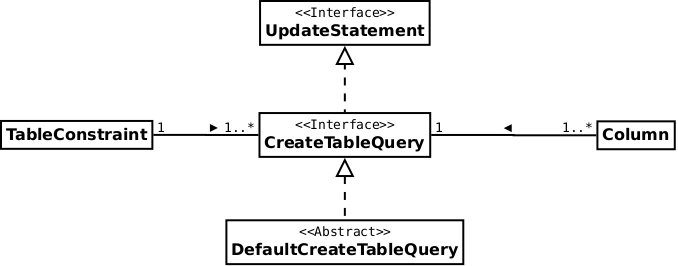
\includegraphics[width=0.7\textwidth]{figuras/jdbgm-dc-createtable.png}
  \caption{Diagrama de clases para la interfaz de CreateTableQuery}
  \label{fig:dc-createtable}
\end{figure}


La clase \verb=TableConstraint= representa a las restricciones de tabla la cual necesita referencias (punteros a los objetos) de las columnas que componen la tabla que se esta por crear y además es posible definir los otros atributos que tienen las restricciones de tabla que se pueden ver en la sección  \fullref{especificacion:dialectos:create}. Lo que no se contemplo en esta interfaz y tampoco es posible definir mediante la misma es el control de la integridad de la sentencia en el sentido de que si es correcta o no pues de hacerlo aumentaría el procesamiento necesario para poder convertir esta sentencia a cadena de caracteres complicando y agregando trabajo extra a la capa de software que accede a el motor, trabajo que en definitiva el terminara realizando de nuevo lo que en definitiva se resumiría en una redundancia innecesaria. Lo único que cambiara al obviar estas comprobaciones es quien terminara por reportar el error por lo que no se realizan este tipo de comprobaciones.

Por ultimo hay que señalar el uso de la clase \verb=Column= para almacenar la definición de las columnas, que además después sera reutilizada como contenedora de valores. Esta clase originalmente contenía las definiciones de las restricciones de columnas pero desde la creación de la clase \verb=TableConstraint= estas fueron eliminadas con la única excepción de la restricción combinada de clave primaria con columna  auto-incrementada del tipo entera.

\subsubsection{La interfaz para UPDATE}
La sentencia \verb=UPDATE= al igual que la sentencia \verb=INSERT= precisa que se le indiquen las columnas sobre las cuales se quiere trabajar, pudiendo ser todas o solo algunas de las columnas, es por ello que se decidió crear una interfaz intermedia que defina este comportamiento para ambas sentencias, dicha interfaz es \verb=UpdateableQuery= la cual precisamente define los métodos necesarios para poder establecer cuales serán las columnas sobre las que se trabajara. Una vista completa de como se disponen las clases necesarias para esta sentencia se puede ver en la figura \ref{fig:dc-updatequery} en ella podemos apreciar que esta interfaz común hace uso de la clase \verb=Column= para almacenar los nombres y valores para las columnas además de los tipos de datos que se precisan para esa columna, aunque como quedo definida la interfaz se deja abierta la posibilidad de que \jj decida a que tipo de dato pertenece el valor que se le acaba de establecer, esto se hace mediante las implementaciones de la interfaz \verb=Formatter= que decide como se debe interpretar el valor de la columna. Y por ultimo antes de entrar directamente a la interfaz especifica para esta sentencia vemos que existe una implementación base para que el comportamiento no solo quede definido sino que también implementado. 

\begin{figure}
  \centering
    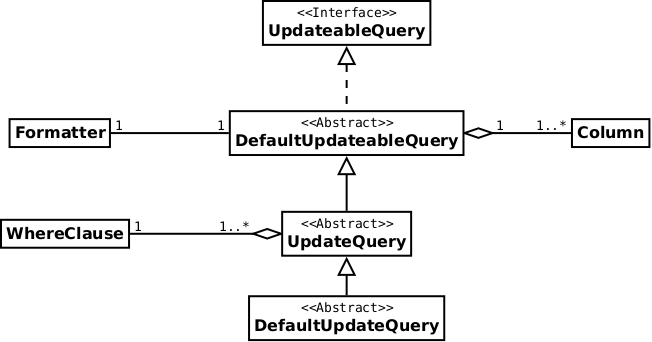
\includegraphics[width=0.7\textwidth]{figuras/jdbgm-dc-update.png}
  \caption{Diagrama de clases para la interfaz de UpdateQuery}
  \label{fig:dc-updatequery}
\end{figure}

Poco le queda por definir a la interfaz \verb=UpdateQuery=, como se puede apreciar en la sección \ref{especificacion:dialectos:update} falta por definir la restricción \verb=WHERE= lo cual se hace mediante la clase auxiliar \verb=WhereClause=, por lo que esta interfaz debe poder devolver un objeto de dicha clase para crear la restricción, este objeto debe ser atributo de la clase que implemente esta interfaz para que luego la clase pueda interactuar con ella y obtener la restricción. 
%El uso de las clases auxiliares y de la interfaz \verb=UpdateableQuery= simplifico mucho a 

\subsubsection{La interfaz para INSERT}

La sentencia \verb=INSERT= como ya se menciono hace uso de la interfaz común \verb=UpdateableQuery= para definir su comportamiento base, luego sera la interfaz \verb=InsertQuery= la que defina el comportamiento especifico para dicha sentencia como se puede observar en la \figpage{fig:dc-insertquery}. En esta interfaz se define el comportamiento especificado en la sección \pageref{especificacion:dialectos:insert}, no hay mas para aclarar con respecto al diseño salvo que esta sentencia puede ser armada a partir de tres fuentes distintas para las cuales existen sendas funciones, como el uso de estas fuentes debe ser excluyentes una de la otra, es decir solo se puede usar una fuente a la vez, se decidió que la interfaz optara como fuente para la sentencia a aquella que haya sido establecida en ultima instancia mediante la llamada a el método correspondiente.

\begin{figure}
  \centering
    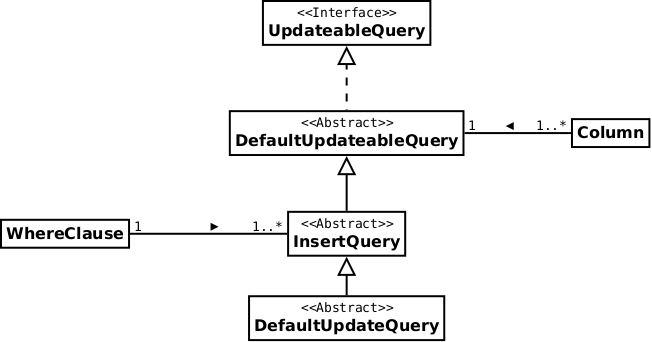
\includegraphics[width=0.7\textwidth]{figuras/jdbgm-dc-insert.png}
  \caption{Diagrama de clases para la interfaz de InsertQuery}
  \label{fig:dc-insertquery}
\end{figure}

\subsubsection{La interfaz para ALTER TABLE}
La sentencia \verb=ALTER TABLE= expresada en la interfaz \verb=AlterTAbleQuery= presenta una estructura bastante simple como se puede ver en la \figpage{fig:dc-altertabletquery} únicamente hace uso de la clase auxiliar \verb=Column= y nada mas tal como se puede apreciar en la sección \ref{especificacion:dialectos:altertable} del capitulo de especificación. Tampoco hay mucho para aclarar debido a la simplicidad de la especificación para dicha sentencia, en parte debido al pobre soporte que tiene sobre esta sentencia el motor \ss y además por que no esta contemplado dentro de lo que serian los métodos CRUD pero como \cc presentaba un soporte para esta se la termino por agregar.
\begin{figure}
  \centering
    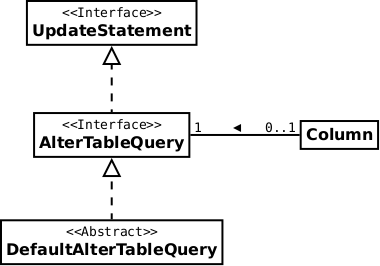
\includegraphics[width=0.5\textwidth]{figuras/jdbgm-dc-altertable.png}
  \caption{Diagrama de clases para la interfaz de AlterTableQuery}
  \label{fig:dc-altertabletquery}
\end{figure}

\subsubsection{La interfaz para DELETE}
La sentencia \verb=DELETE= definida en la interfaz \verb=DeleteQuery= es otra de las que es bastante sencilla según la especificación dada en la sección \fullref{especificacion:dialectos:delete} en la que se ve que aparte del nombre de la tabla sobre la que se esta trabajando necesita de una clausula \verb=WHERE= la cual es proveída por la clase \verb=WhereClause= tal como se puede ver en la \figpage{fig:dc-deletequery}.

\begin{figure}
  \centering
    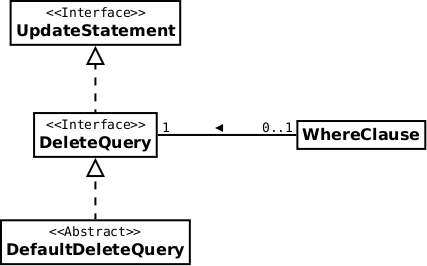
\includegraphics[width=0.5\textwidth]{figuras/jdbgm-dc-delete.png}
  \caption{Diagrama de clases para la interfaz de DeleteQuery}
  \label{fig:dc-deletequery}
\end{figure}

\subsubsection{La interfaz para SELECT}
La sentencia \verb=SELECT= definida en la interfaz \verb=SelectQuery= es la mas complicada de todas con las que se estuvo trabajando, para no sobrecargarla muchas de las tareas se relegaron  a clases auxiliares, la primera de ellas es la clase \verb=WhereClause= que ya se había utilizado previamente para crear restricciones del tipo \verb=WHERE=, la segunda clase auxiliar que fue creada exclusivamente para esta sentencia es la clase \verb=JOIN= que se encarga de ofrecer los métodos necesarios para establecer las restricciones de origen \verb=FROM=. La clase que se podría haber utilizado pero que no se usa es \verb=Column= puesto que para \verb=SELECT= lo que realmente importa es el nombre de la columna y quizá un alias y nombre de la tabla de la misma, pero estos datos no justifican el uso de \verb=Column= por lo que se decidió no usar la misma.

\begin{figure}
  \centering
    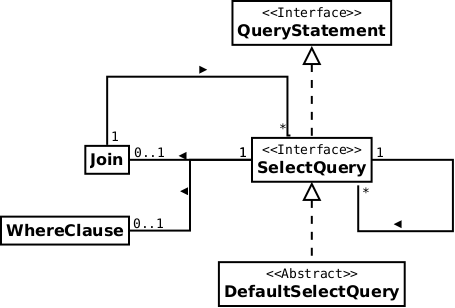
\includegraphics[width=0.5\textwidth]{figuras/jdbgm-dc-select.png}
  \caption{Diagrama de clases para la interfaz de SelectQuery}
  \label{fig:dc-selectquery}
\end{figure}

En la figura \ref{fig:dc-selectquery} se puede ver el diagrama de clases para \verb=SELECT= en el que se puede ver que la clase hace uso de si misma y además \verb=Join= también hace uso de la misma, pues es posible hacer \verb=UNION= con otra sentencia \verb=SELECT=, la clase \verb=Join= también hace uso de esta interfaz por que se la puede usar como sentencia anidada dentro de una restricción \verb=JOIN=. Otro punto importante dentro de esta clase es el soporte de las funciones agregadas de las bases de datos, estas como ya se dijo no son parte del estándar y por lo tanto se encuentra disparidad ente ellas, por lo que se opto que las funciones se podrán elegir desde un catalogo de constantes disponibles en la clase \verb=Functions= que proveerá nombres de funciones que tienen equivalentes en los tres motores quedando a cargo del programador el correcto uso de la misma.

\subsection{Controlando la creación de objetos}

Observando la estructura que se fue proponiendo hasta ahora tenemos una tres implementaciones concretas por cada una de las interfaces que definen a las diferentes sentencias, una por cada motor al que se le da soporte, así que con lo expuesto hasta ahora el programador debe decidir cual es la implementación que necesita usar y en base a ello instanciar siempre las del mismo tipo teniendo en cuenta el motor que se quiere usar. Siguiendo esta lógica el código resultante puede resultar difícil de mantener, obstruyendo el objetivo primordial de \jj,  pues en el momento que se desea migrar de motor sera necesario buscar una por una las variables que se fueron declarando para las sentencias SQL para corregir el tipo con el que fueron declaradas y además cambiar a el constructor adecuado o también puede ocurrir que el programador haya usado correctamente como tipo de dato para las variables a su correspondiente interfaz en cuyo caso aun restaría por corregir el uso del constructor adecuado. Así que para sortear este problema se hará uso de el patrón \textit{Abstract Factory}

\subsubsection{El patrón Abstract Factory}
Podemos decir en forma resumida que el patrón Abstract Factory le permite a un cliente crear objetos que son parte de una familia de objetos relacionados o dependientes. El tema o rasgo en común de esta familia de objetos puede llegar a ser pertinente a muchas mas clases por lo que en estos casos se suele crear paquetes paralelos que mantienen separadas estas familias de objetos dependiendo de como las afecte el rasgo en común. Una clase que implemente este patrón le provee a una clase cliente una fabrica que le permite crear objetos que están relacionados mediante un rasgo en común. Una descripción mucho mas detallada y sencilla de comprender puede ser encontrada en el siguiente libro\cite{Metsker:2002:DPJ}. 

%The ABSTRACT FACTORY pattern lets you arrange for a client to create objects that are part of a family of related, or dependent, objects. The theme, or common trait of the family, such as which country the classes pertain to, may run across many classes. In this case, you may maintain parallel packages, perhaps placing each family in its own package. For GUI factories, you may not need more than one package if different "classes" of GUI components differ only in such attributes as text size and cursor type. However you organize your code, ABSTRACT FACTORY lets you provide a client with a factory that produces objects that are related by a common theme.
Bajando un poco el nivel de abstracción podemos ver que para que las diferentes familias de clases estén relacionadas estas deben implementar u heredar de una interfaz o clase abstracta en común, entonces una implementación posible de este patrón consiste en crear una interfaz Fabrica que defina métodos para obtener las implementaciones de cada una de las interfaces de la familia, de este modo cada una de las familias implementara esta interfaz Fabrica para devolver instancias de objetos que se correspondan con su familia, utilizando siempre como tipo a las interfaces que definen a la familia. Con esto se obtendrán tantas Fabricas especificas como familias existan por lo que resta obtener la fabrica adecuada dependiendo de la variable externa que hace de tema común para la familia. el concepto quedara mas claro cuando se exponga el modo en que fue implementado el patrón en este caso.
 
\subsubsection{Implementación del patrón}

En el manejador de sentencias las familias vendrían a estar formadas por el conjunto de implementaciones de las interfaces que definen las sentencias SQL soportadas y habría una familia por cada motor al que se le este dando soporte, para estas el tema en común seria precisamente el motor en especifico que se este usando. Viéndolo desde otro punto de vista dependiendo de el motor en particular que estemos usando deberemos instanciar objetos de una familia determinada. Algo que queda un poco implícito con el uso de este patrón es que una vez que se tiene la ``fabrica'' adecuada ya no es necesario preocuparse por que tipo de objetos se esta instanciando y si se usan como tipo de datos a las interfaces, para cambiar de motor lo único que se tiene que hacer es cambiar de ``fabrica''.

En este proyecto la clase que se encargara de implementar el patrón Abstract Factory sera \verb=SQLFactory=, que tiene que realizar dos tareas principales: primero se encargara de definir métodos abstractos para devolver instancias de las diferentes clases que implementen las interfaces base; segundo se encargara de decidir de cual familia de clases se deben instanciar los objetos. Para la segunda tarea la clase deberá verificar si es que ya se estableció con que motor se desea trabajar y en base a esto decidir que implementación especifica de la clase \textit{factory} debe trabajar, pues la razón de definir como clase abstracta a \verb=SQLFactory= es que los métodos abstractos de la misma sean implementados en clases especificas para que estas devuelvan el tipo adecuado de objetos, esto se puede apreciar mejor en la figura \ref{fig:crossdb-factory} que sintetiza lo que se vino explicando. 

\begin{figure}
  \centering
    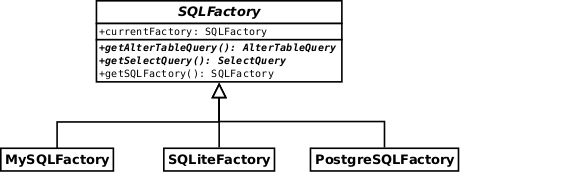
\includegraphics[width=0.85\textwidth]{figuras/crossdb-factory.png}
  \caption{Diagrama de clases para las clases ``Fabrica''}
  \label{fig:crossdb-factory}
\end{figure}

En dicha figura no se muestran todos los métodos abstractos que debe tener \verb=SQLFactory= pero debe existir uno por cada interfaz base y siguiendo el mismo molde \verb=get[Interfaz](): Interfaz=, el método de clase \verb=getSQLFactory()= debe verificar que se haya establecido el motor con el cual se quiere trabajar para poder decidir de que implementación se debe instanciar. Las clases que implemente a la fabrica lo único que deben hacer es implementar de forma adecuada los métodos abstractos.  

\section{Capa de acceso a el motor - JDBC}
Una vez diseñado el manejador de sentencias es necesario diseñar la capa que se encargara de abstraer el uso de \jd, esta capa como ya se menciono trabajara las sentencias SQL con el formato propuesto en el manejador de sentencias de modo que obligara el uso del mismo en pos de mantener la compatibilidad. La principal tarea de esta capa será la de ocultar el uso de \jd  a la vez que se ofrece una interfaz mucho mas simple y fácil de usar junto con pre-configuraciones para poder usarlo sin necesidad de muchas configuraciones. En orden de establecer el diseño para esta capa es necesario entender algunos puntos importantes en el funcionamiento de la API que se esta ocultando.

\subsection{Como funciona JDBC}
\jd es un API bastante completo para poder acceder, según su documentación, virtualmente a cualquier tipo de datos tabulares contándose entre estos a las bases de datos relacionales, el flujo de trabajo minimo cuando se usa \jd se puede resumir en los siguientes pasos:

\begin{enumerate}
\item Establecer una conexión. %Establishing a connection.
\item Crear un \verb=statement=. % Create a .
\item Ejecutar una consulta. %Execute the query.
\item Procesar el objeto. \verb=ResultSet=. %Process the ResultSet object.
\item Cerrar la conexión. %Close the connection.
\end{enumerate}

Para \textbf{establecer la conexión} con la  fuente de los datos, una BD relacional en este caso aunque puede tratarse de otros medio, es necesario contar con el \textit{driver} jdbc adecuado para poder obtener un objeto de la clase \verb=Connection= que es la que representara la conexión después de esto mediante la conexión ya se puede \textbf{crear un objeto de} \verb=Statement= que es una interfaz que representa sentencias SQL "vacias" y brinda diferentes métodos para poder \textbf{ejecutar} sentencias sobre el motor, existen tres tipos \verb=Statement, Preparedstatement= y \verb=CallableStatement= siendo estas dos ultimas extensiones de la primera. Una vez ejecutada la sentencia, dependiendo del tipo de sentencia que se haya ejecutado se, se obtienen resultados como \verb=int= o \verb=ResultSet= que es la que interesa pues da acceso a los datos que son resultado de la consulta mediante un cursor para ir obteniendo fila por fila los datos obtenidos, por ultimo una vez que se obtuvieron o modificaron los datos necesarios es necesario liberar los recursos mediante los métodos \verb=close()= que ofrece \verb=Statement= para liberar los recursos de la consulta y \verb=Connection= para terminar la conexión con la base de datos lo cual cierra completamente la comunicación con el motor, mientras que el método anterior libera los recursos usados por la consulta\citep{java:jdbc:tutorial}.

Para entender un poco mejor el funcionamiento se analizara una porción de código mínima que ilustra el uso de esta API y muestre que al hacer uso de el es necesario hacer algunas configuraciones especificas que pueden ser ``automatizadas''.

\begin{lstlisting}[title=Porción de código java para la conexión a una base de datos]
class conectDB(){
...

	Class.forName("com.mysql.jdbc.Driver");
	Connection conexion = DriverManager.getConnection(
		"jdbc:mysql://localhost/AsistenciaAlumnos", "tester",
		"tester");
	Statement st = (Statement) conexion.createStatement();
	String query = "SELECT * FROM tabla";
	ResultSet rs = stmt.executeQuery(query);
	while (rs.next()) {
		String coffeeName = rs.getString("COF_NAME");
		System.out.printline(coffeeName);
	}
	rs.close();

...
}
\end{lstlisting}

En esta porción de código lo que se hace inicialmente es instanciar el driver el cual es necesario que exista para poder obtener una conexión a la BD, es decir crear el objeto driver, luego el método estático \verb=DriverManager.getConnection()= nos devuelve un objeto que representa la conexión al motor con el que se esta trabajando. Este objeto del tipo \verb=Connection= nos provee métodos para generar los objetos \verb=Statement= que nos permite hacer consultas a la base de datos mediante las funciones que dispone como por ejemplo el método \verb=executeQuery()= que nos permite hacer consultas del tipo \verb=SELECT= y que como resultado devuelve un objeto \verb=ResultSet= del que se pueden ir extrayendo fila por fila los datos obtenidos. Los objetos \verb=ResultSet= y \verb=Statement= estan sumamente relacionados por ejemplo si se cierra una sentencia mediante \verb=Statement.close()= el \verb=ResultSet= obtenido de la misma también sera cerrado y además solo pueden existir en una relación uno a uno. Una descripción mucho mas extensa de JDBC puede ser encontrada en la documentación disponible en la web de Oracle\citep{java:jdbc}.

\subsection{El diseño}
La API que ofrecerá \jj sera sencillo para simplificar el uso de \jd, tal  como se comento en el capitulo \ref{capitulo:especificacion} este debe ofrecer métodos para realizar consultas y manejar la conexión con el motor, así que para generalizar el API se creara una interfaz para definirla, la cual tendrá una única implementación base, al menos para este caso, la cual deberá tener implementaciones especificas para cada uno de los motores.

\begin{figure}
  \centering
    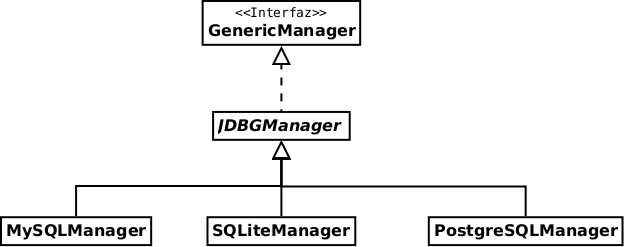
\includegraphics[width=0.85\textwidth]{figuras/jdbgm-jdbc.png}
  \caption{Diagrama de clases para la capa de abstracción de JDBC}
  \label{fig:jdbgm-jdbc}
\end{figure}

En la figura \ref{fig:jdbgm-jdbc} se puede ver mas claramente la estructura elegida para la capa de abstracción, en esta podemos ver la interfaz que se encarga de definir la API en \verb=GenericManager= la cual puede parecer que es innecesaria pero si tenemos en cuenta que en el futuro se puede usar una interfaz diferente de \jd para acceder a los motores toma algo de sentido la existencia del mismo aparte la interfaz hace mucho mas clara la lectura de los métodos disponibles. La clase abstracta \verb=JDBCManager= es la implementación de la interfaz anterior haciendo uso de \jd en la que se deben implementar todos los métodos definidos puesto que en lo que diferenciaran las implementaciones especificas es valga la redundancia en configuraciones especificas para cada uno de los motores, estas diferentes implementaciones entonces únicamente deberán darle valores específicos para los atributos no configurables como por ejemplo el nombre de el driver.

\subsection{Manejo de errores y excepciones}
Un importante tema a tener en cuenta en esta parte de el proyecto es el manejo de errores, en \jd casi todos los métodos son capaces de lanzar excepciones del tipo \textit{checked exceptions} los cuales deben ser capturados o bien lanzados nuevamente por el método que lo recibió caso en cual el método deberá ser marcado con la palabra reservada \verb=throw= del modo siguiente \verb=metodo() throws Exception=. Como \jj esta echo para escribir mas código sobre el, este no puede decidir concretamente que hacer cuando ocurren las excepciones a diferencia de lo que ocurre con el manejador de sentencias donde todos los errores que se pueden producir son del tipo \textit{unchecked exceptions} que interrumpen la ejecución de el programa en esta sección los errores deben ser capturados y tratados pero no por \jj si no por el que este haciendo uso de el mismo y es por eso que las excepciones que debe lanzar \jj deben ser también del tipo \textit{checked exceptions}.

Como la fuente de las excepciones en este caso es \jd todas las excepciones que lancen los métodos de el API de la capa de acceso a el motor serán básicamente errores que envuelven a los  errores que devuelve \jd que son del tipo \verb=SQLException= o alguna subclase de la misma. Para ellos se creara la clase \verb=JDException= la cual sera una subclase de \verb=Exception= que es la clase base para este tipo de excepciones, como la principal tarea de nuestra excepción es la de servir de envoltorio para las excepciones que puedan ser lanzadas por los métodos subyacentes la misma debe contar con un atributo del tipo \verb=SQLException= para contenerlas, además como los métodos de este API ocultan el uso de mas de una función cada uno de los cuales puede lanzar un error por diferentes razones \verb=JDException= ah de tener información extra con respecto al método donde se produjo el error. Una vista abstracta de estas clases las podemos ver en el diagrama \ref{fig:jdbgm-exception}.

\begin{figure}
  \centering
    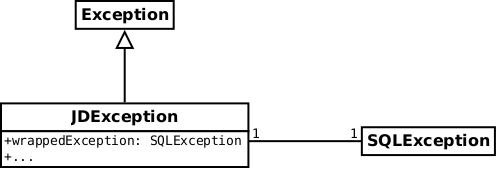
\includegraphics[width=0.7\textwidth]{figuras/jdbgm-exception.png}
  \caption{Diagrama de clases para JDException}
  \label{fig:jdbgm-exception}
\end{figure}

Como la información extra que tiene \verb=JDException= concierne mas a la capa que esta presente en \jj la información de muchos de las excepciones que interesen al programador estarán en la clase \verb=SLQException= este deberá conocer la información que este contiene, una descripción de los mismos puede ser encontrado en la web de Oracle\citep{java:exeptions}, y la cual debe ser conocida por el programador si es que no es suficiente la información que brinda explícitamente \verb=JDException= por lo que deberá acceder a la excepción que esta siendo envuelta para poder obtener más información.

\subsection{Que se devuelve como resultado}
Al ejecutar las sentencias SQL sobre el motor es posible obtener uno de dos tipos de resultados posibles dependiendo de si son consultas (\verb=SELECT=) las cuales devuelven un tipo de dato complejo representado por la clase \verb=ResultSet= que representa la tabla resultado de la consulta o bien un tipo de dato primitivo \verb=int= para las otras sentencias que usualmente indica la cantidad de filas que fueron afectadas por la sentencia salvo para el caso de las sentencias del tipo DDL que no afectan a las filas de datos.

Cuando el tipo de datos devuelto es \verb=int= no hay mucho para decir salvo que ese mismo valor sera devuelto por nuestro API, para el caso de \verb=ResultSet= también sera devuelto el mismo objeto pero por que como \jj no esta implementando un \verb=ORM= es necesario un modo de extraer los datos de la BD y esto esta brindado por \verb=ResultSet= de una manera bastante completa por lo que proveer un método propio para extraer los datos seria como envolver los métodos de dicha clase sin ningún añadido por lo que estaríamos frente a una clase que lo único que hace es renombrar los métodos de \verb=ResultSet=, por otro lado esta clase es implementada por el proveedor del driver por lo que es "independiente" de un motor en especifico, salvo que existan implementaciones que mal interpretaron las interfaces de \jd pero dicho caso es bastante improbable.